
\chapter{Responsive Information Visualization}
\label{chap:ResponsiveInformationVisualization}

A \emph{responsive} visualization is a visualization which adapts
itself to the available display space and properties of the device
used to access it. Analogous to responsive web design, the need for
responsive visualizations arises from the growing variety of devices
used to consume content and the physical differences between them.
Visualizations and charts often form significant blocks of content
embedded inside web pages. For a web page to be responsive, any
embedded content such as visualizations and charts must also be
responsive.

Visual elements require proper sizing and spacing to be of
value. Merely scaling visualizations to fit into their allocated space
is insufficient to provide a seamless experience to users, as has
already been discussed in Section~\ref{sec:RWD}. Another factor which
is often ignored is the different methods of interaction inherent to
specific types of devices, such as touch and keyboard interaction. For
example, to ensure that data points remain selectable on less precise
input devices such as touchscreens, a visualisation might adapt by
reducing the data density and increasing the size of individual
elements. The goal of responsive visualizations is that they should
adapt themselves to the characteristics of the consuming device and
context so as to remain as effective and usable as possible
\parencite{DesignPatternsTradeOffsRespVis}.


The topic of responsive visualization only gained prominence in recent
years, as responsive web design became mainstream.
\textcite{BuildingRespDataVisForTheWeb} used the term responsive
visualization, but only descibed how to implement scalable
visualizations. \textcite{LearningRespDataVis} covered scalable
visualizations, but also considered interactive selection and touch
events. \textcite{RespVis} was possibly the first academic work to
address design patterns for responsive visualization.
%
More recently, \parencite{TechniquesForFlexibleRespVisDesign} surveyed
the design space of responsive visualizations, created a taxonomy of
currently used techniques and recurring patterns, and presented a tool
to help design responsive visualisations side-by-side. In addition to
surveying design patterns, \textcite{DesignPatternsTradeOffsRespVis}
also consider issues around different forms of \enquote{message loss}
when reducing chart complexity, and define optimization of the
density-message trade-off as one of the main challenges when designing
responsive visualizations.

One of the most current works summarizing much of the research
surrounding responsive visualizations is
\textcite{Lee-2021-Mobile-Vis}. Chapter~2 about responsive
visualization design \parencite{Horak-2021-Responsive-Vis} is of a
particular interest for this work as it gives a quite complete summary
on the research in this field. It discusses the differences between
responsive web design and responsive visualization design and stresses
that visualizations must not be seen as mere images embedded in a
website but that they must adapt to device characteristics to deliver
a satisfactory user experience. Furthermore,
\textcite{Horak-2021-Responsive-Vis} continue to go into details about
various factors affecting a visualization's responsive design and give
an overview of high-level design strategies (called design patterns in
this work) for responsive visualizations. Lastly, unique challenges
and opportunities for responsive visualization design are summarized
to guide researchers to potentially interesting topics for future
research in this area.


\section{Responsive Visualization Patterns}

Patterns are templates for solving recurring problems.
\textcite{TechniquesForFlexibleRespVisDesign} created a comprehensive
taxonomy of responsive techniques, as well as a tool to help design
responsive visualisations side-by-side. They proposed describing
responsive techniques according to five \emph{actions}, which are
applied to different components. These actions are: (1) resize, (2)
reposition, (3) add, (4) modify and (5) remove. A sixth action refers
to leaving a component unchanged, but this is deemed a non-technique
and therefore left out here. They also described a non-exhaustive set
of eleven \emph{components}, upon which these actions can be
performed: (1) axis, (2) axis labels, (3) axis ticks, (4) gridlines,
(5) legend, (6) data, (7) marks, (8) labels, (9) title, (10) view, and
(11) interaction. It should be noted that some combinations of actions
and components do not make sense and therefore do not occur in
practice. It is, for example, not possible to resize interactions or
reposition data.  \textcite{TechniquesForFlexibleRespVisDesign}
performed their research following a desktop-first approach of
responsive design, because the interviews they conducted with
visualization authors revealed a strong inclination towards this
approach. They found that when adapting desktop visualizations for
narrow screens, it was much more common to remove elements (37.7\%)
than to add them (11.3\%). Another interesting finding was that most
visualizations (88.7\%) implemented no change at all for their
interactions, while some (10\%) even removed interactive capabilities
completely. Only very few visualizations (5.6\%) improved the
experience of mobile users by adapting interactions accordingly.



The most detailed research on patterns in responsive visualization
design was performed by \textcite{DesignPatternsTradeOffsRespVis}.
Following \textcite{TechniquesForFlexibleRespVisDesign}, they
characterised the responsive visualization strategies according to
(the same) two dimensions: \emph{targets}, representing what entity is
changed, and \emph{actions}, representing how entities are changed.
However, the targets and actions are more finely grained, having a
number of sub-categories.
%
Targets are grouped into five distinct categories (Data, Encoding,
Interaction, Narrative, and References/Layout), with four of the five
categories further divided into sub-categories, as shown in
Table~\ref{tab:PatternsTargets}.
%
Actions are also grouped into five distinct categories (Recompose,
Rescale, Transpose, Reposition, and Compensate), with four of the five
top-level categories again having sub-categories, as shown in
Table~\ref{tab:PatternsActions}. The actions are defined as operations
with distinct input and output states to ensure they can be inverted,
and thus can be applied to either desktop-first or mobile-first design
approaches
%
Categorizing techniques using these dimensions, the authors identified
a total of 76 viable strategies, whereby some of them are not used in
the visualizations they studied. Their explorable online gallery
\parencite{DesignPatternsTradeOffsRespVisGallery} contains examples
demonstrating all the patterns they discovered.


\begin{table}[tp]
\tablestretch
\rowcolors{2}{}{tablerowcolour}
\centering
\begin{tabularx}{\linewidth}{>{\kern-\tabcolsep}l>{\raggedright}p{0.2\textwidth}X<{\kern-\tabcolsep}}
\toprule
Category & Targets & Description \\
\midrule
Data & Records, Fields, Level & Data is the information which is encoded in a visualization. \\
Encoding & & Encodings are the visual forms in which data is represented. \\
Interaction & Feature, Trigger, Feedback & Interactions define how users can engage with visualizations. \\
Narrative & Sequencing, Annotations, Emphases, Text & This category groups targets based on the story a visualization should convey. \\
References/Layout & Labels, References, Layout, Size & References represent additional information which makes visualizations easier to understand, and a layout describes how the individual visual components are placed. \\
\bottomrule
\end{tabularx}
\caption[Targets of Responsive Visualization Patterns]{
The targets of responsive visualization patterns identified by
\textcite{DesignPatternsTradeOffsRespVis}.
\imgcredit{Table adapted from \textcite{DesignPatternsTradeOffsRespVis}.}
}
\label{tab:PatternsTargets}
\end{table}




\begin{table}[tp]
\tablestretch
\rowcolors{2}{}{tablerowcolour}
\centering
\begin{tabularx}{\linewidth}{>{\kern-\tabcolsep}l>{\raggedright}p{0.3\textwidth}X<{\kern-\tabcolsep}}
\toprule
Category & Actions & Description \\
\midrule
Recompose & Remove, Add, Replace, Aggregate & Actions which affect the existence of targets. \\
Rescale &  & Actions which affect the size of targets. \\
Transpose & Serialize, Parellelize, Axis-Transpose & Actions which affect the orientation of targets. \\
Reposition & Externalize, Internalize, Fix, Fluid, Relocate & Actions which affect the position of targets. \\
Compensate & Toggle, Number & Actions which compensate for loss of information. \\
\bottomrule
\end{tabularx}
\caption[Actions of Responsive Visualization Patterns]{%
The actions of responsive visualization patterns identified by
\textcite{DesignPatternsTradeOffsRespVis}.
\imgcredit{Table adapted from \textcite{DesignPatternsTradeOffsRespVis}.}
}
\label{tab:PatternsActions}
\end{table}



\section{Responsive Visualization Examples}

The goal of this section is to provide the reader with some
demonstrative examples of responsive visualizations. Due to the
complexities of using images from commercial websites, the figures in
this section were taken from external academic sources from which
permissions are more straightforward to procure. These responsive
visualizations put most of their effort into demonstrating responsive
patterns rather than communicating messages in their data, and owing
to this, some of them lack essential features, such as titles and axes
descriptions, usually present in practice. For more real-life examples
of responsive visualizations,
\textcite{DesignPatternsTradeOffsRespVisGallery} should be consulted. 

The examples in this section are organized by chart type. It would be
an immense endeavor to bring examples for every pattern used for all
types of charts, so only a subset which demonstrates some of the most
frequently encountered patterns for frequently used types of charts is
summarized here. The popularity of chart types was judged using the
responsive visualization corpus collected in
\textcite{DesignPatternsTradeOffsRespVisGallery} and the visualization
corpora from the Quarz news website and academic papers collected by
\textcite{ReverseEngineeringVisualizations}. Both of these sources
lead to the conclusion that line charts, bar charts, and point charts
are the most frequenly occuring types of visualizations.





\subsection{Bar Charts}
\label{sec:BarChartExamples}

Bar charts are usually used to visualize two-dimensional data, with
one categorical dimension and one quantitative dimension. Two variants
of bar charts support the visualization of categorical datasets having
subdimensions: grouped bar charts \parencite{GroupedBar} compare
subdimensions with each other, and stacked bar charts
\parencite{StackedBar} compare part-to-whole relationships of the
subdimensions. Even though responsive design of visualizations is
slowly becoming more common, most charts found in today's web articles
are still created as static images
\parencite{HBar,VBar,HVBar,MapBarLine}.

A good example of a responsive bar chart can be seen in
Figure~\ref{fig:RespBarExample} \parencite{RespVis}. Bar charts are
freely scalable by adjusting the width of individual bars
\parencite{RespHBar,RespHBarHLine,RespHBars}, so they all can fit into
their allocated space. When reducing the width of any type of chart
past a certain point, the tick labels of the horizontal axis may start
to overlap. This is why the reducing width pattern usually occurs
together with the recompose axis ticks and simplify/elaborate axis
labels patterns \parencite{RespHBars,RespHBarHLine,RespVBar}. Another
effective pattern for avoiding overlapping tick labels is to rotate
the labels by up to 90 degrees so they take up less horizontal space
\parencite{RespVis}. If there is too much data to fit into the
available width, the chart can be transposed and grown to as much
height as is required necessary \parencite{RespVis}. Doing this is
more advisable than simply extending the width of the chart past the
viewport, since vertical scrolling is easier than horizontal
scrolling. When reducing the width of charts containing annotations, a
number of patterns can be applied to avoid annotations
overlapping. For example, annotations can be removed
\parencite{RespHStackedBar,RespHLineHStackedBar}, simplified, or
relocated \parencite{RespVBar}.



\begin{figure}[tp]
\newlength{\respbarwidth}
\setlength{\respbarwidth}{0.95mm}
\centering
\subfloat[][%
70rem
]
{%
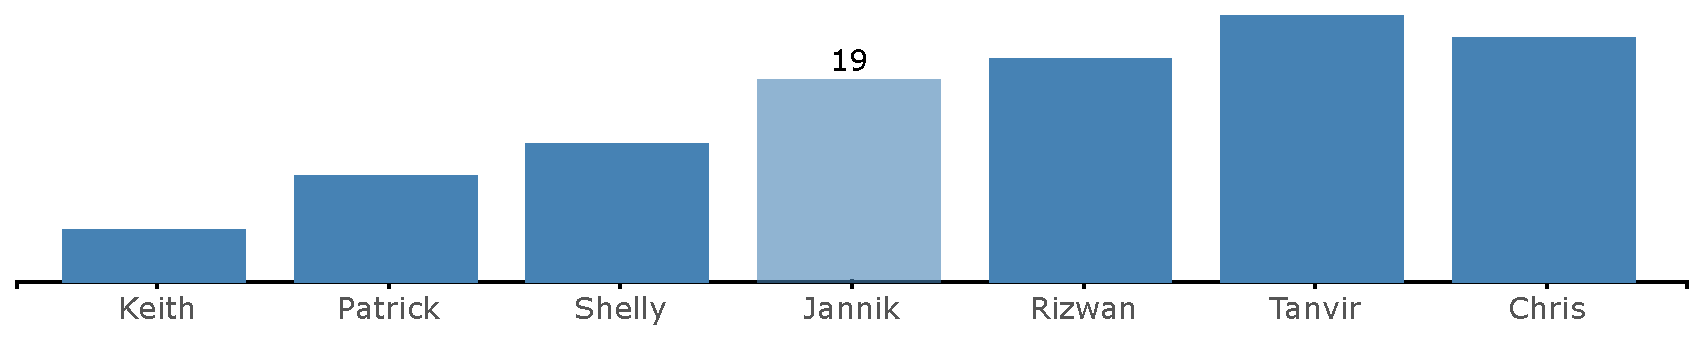
\includegraphics[width=70\respbarwidth]
{diagrams/resp-bar-1.pdf}%
\label{fig:RespBarExample1}%
}
\hfill
\subfloat[][%
50rem
]
{%
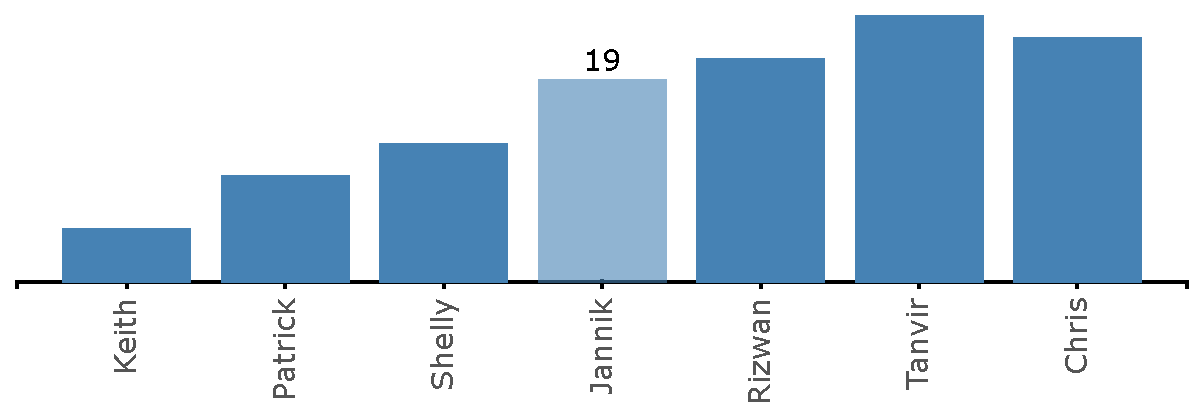
\includegraphics[width=50\respbarwidth]
{diagrams/resp-bar-2.pdf}%
\label{fig:RespBarExample2}%
}
\hfill
\subfloat[][%
30rem
]
{%
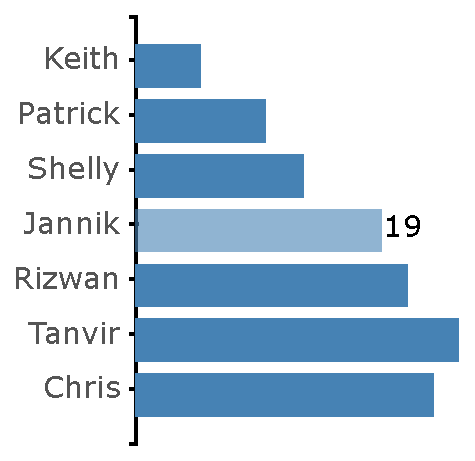
\includegraphics[width=30\respbarwidth]
{diagrams/resp-bar-3.pdf}%
\label{fig:RespBarExample3}%
}
\caption[Responsive Bar Chart Example]
{
A responsive bar chart at different display widths.
\subref{fig:RespBarExample1} At 70rem, axis tick labels are aligned
horizontally. \subref{fig:RespBarExample2} At 50rem, axis tick labels
are aligned vertically. \subref{fig:RespBarExample3} At 30rem, the
chart is transposed.
\imgcredit{Screenshots of \textcite{RespVis} created by the author of
  this thesis. Used with kind permission by Keith Andrews.}
}
\label{fig:RespBarExample}
\end{figure}






\subsection{Line Charts}
\label{sec:LineChartExamples}

Line charts are used to show trends in two-dimensional
datasets by plotting them as points connected by lines (a polyline).
They can be extended to compare trends in an additional categorical
dimension by drawing additional polylines for each category. Many line
charts on the web are published in non-responsive forms
\parencite{HLine,HLine2}, although some authors take the extra effort
to make their charts responsive. The minimum which can be done to make
a line chart responsive is to reduce their width
\parencite{RespRadialScatterHLine} on narrower screens by shrinking
the horizontal distance between neighboring points. This usually
occurs together with the recomposition and simplification of
horizontal ticks. If the chart contains annotations, it may also be
necessary to recompose, relocate, and simplify them as well
\parencite{RespHLines,RespHLine,RespHBarHLine,RespHLineHStackedBar}.

A good demonstration of which responsive patterns can be applied to
make a line chart responsive is shown in the responsive line chart
created by \textcite{RespVis} which can be seen in
Figure~\ref{fig:RespLineExample}. In addition to the recomposition of
ticks, tick labels are rotated to reduce their required horizontal
space. For exceptionally limited space, it can make sense to remove
the axes of a line chart entirely and turn it into a sparkline.
However, it should be noted that by doing this, the consumer of the
visualization loses information about the type and scale of the
chart's dimensions. This technique should therefore only be applied in
cases where no other pattern is applicable or if the trend in the data
is the most important message to convey. It is rare to encounter
transposed versions of line charts, although transposition could
sometimes benefit heavily annotated line charts \parencite{VLine}.
Applying a transpose pattern would allow the chart to take up as much
vertical space as necessary to neatly accomodate annotations without
requiring the consumer to scroll horizontally.



\begin{figure}[tp]
\newlength{\resplinewidth}
\setlength{\resplinewidth}{1.15mm}
\centering
\subfloat[][%
65rem
]
{%
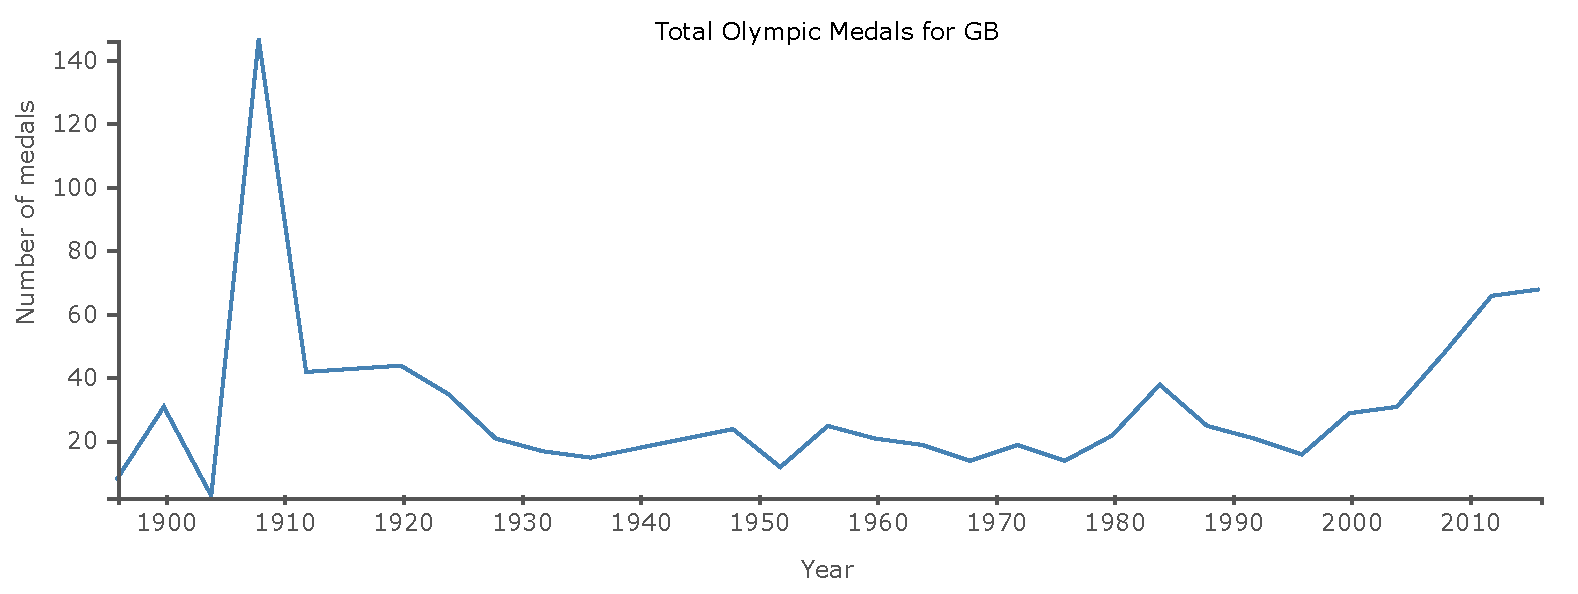
\includegraphics[width=65\resplinewidth]
{diagrams/resp-line-1.pdf}%
\label{fig:RespLineExample1}%
}
\hfill
\subfloat[][%
40rem
]
{%
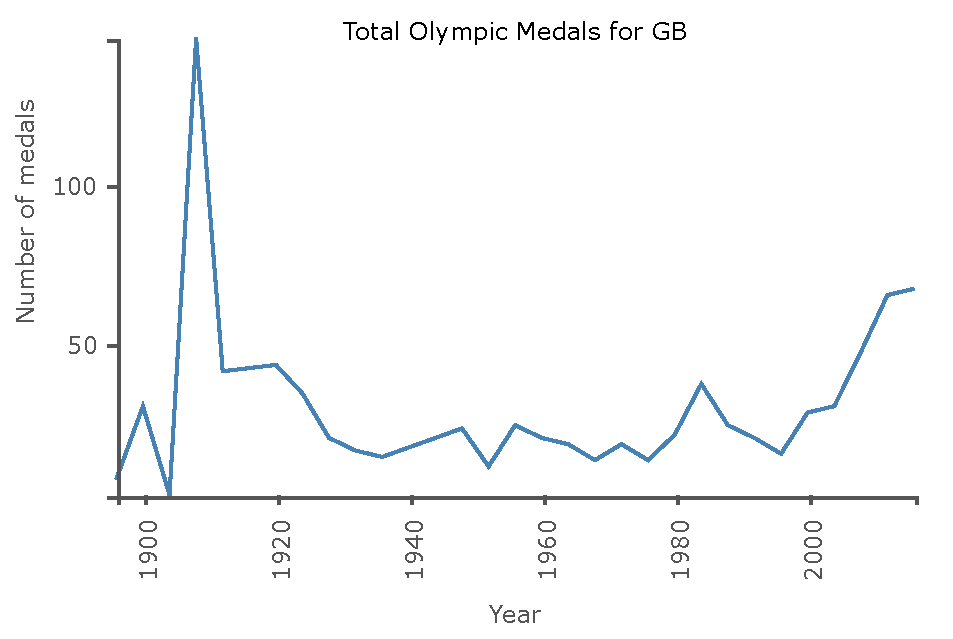
\includegraphics[width=40\resplinewidth]
{diagrams/resp-line-2.pdf}%
\label{fig:RespLineExample2}%
}
\hfill
\subfloat[][%
20rem
]
{%
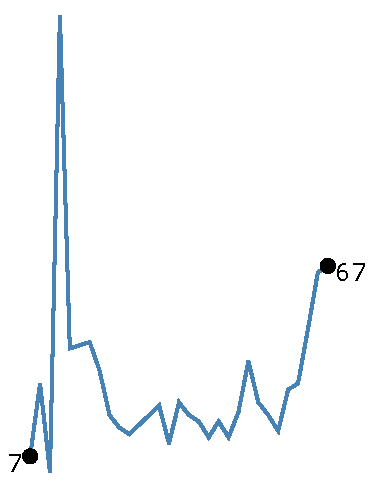
\includegraphics[width=20\resplinewidth]
{diagrams/resp-line-3.pdf}%
\label{fig:RespLineExample3}%
}
\caption[Responsive Line Chart Example]
{
A responsive line chart at different display widths.
\subref{fig:RespLineExample1} At 65rem, the x axis labels are
horizontal.  \subref{fig:RespLineExample2} At 40rem, the x axis ticks
have been thinned out and the labels fully rotated by 90\textdegree.
\subref{fig:RespLineExample3} At 20rem, both axes have been removed,
and the chart has become a sparkline.
\imgcredit{Screenshots of \textcite{RespVis} created by the author of
  this thesis. Used with kind permission by Keith Andrews.}
}
\label{fig:RespLineExample}
\end{figure}









\subsection{Point Charts}
\label{sec:ScatterplotExamples}

Point charts, also known as scatterplots, represent data as points in
2d Cartesian coordinate systems. There are many examples of
point charts published as static images \parencite{Scatter,Scatter2},
with responsive versions starting to emerge. The first step to making
point charts responsive is to reduce their width to fit them into the
space available. As for other types of charts, care must be taken to
avoid overlapping of labels and annotations by applying recomposition,
relocation and simplification patterns
\parencite{RespScatter,RespScatter2}. To counteract the increased
density of points when reducing the size of their container, various
interaction features are usually implemented in point charts to aid
consumers in interpreting the represented data. The most useful
interaction features in these charts are elaborative zooming
interactions and the explorative panning interactions. In addition to
zooming and panning, \textcite{RespVis} employs additional methods to
ameliorate the overlapping of individual points, including fisheye
distortion, Cartesian distortion, and temporary displacements of
points.

An interesting technique for responsive point charts based on the
visualization's density (data points per pixel) rather than its width
was introduced by \textcite{NickRabinowitzRDV}. The benefit of this
approach is that charts adapt to changing amounts of data and
reconfigure their appearance accordingly. The patterns applied in the
responsive point chart shown in Figure~\ref{fig:RespScatterExample}
are the recomposition of annotations to only show annotations for
selected data records, and the switching of the encoding from a point
chart to a heatmap for high point densities. Other techniques, such as
the recomposition of data records, would also be applicable to
responsive point charts, but no examples for such patterns could be
found. If the data to be encoded is inherently cyclic, a radial point
chart, using polar coordinates, can be used to better reflect the
cyclic nature of the data \parencite{RespRadialScatterHLine}.



\begin{figure}[tp]
\centering
\subfloat[][%
Low density % (0.00005 points per pixel).
]
{%
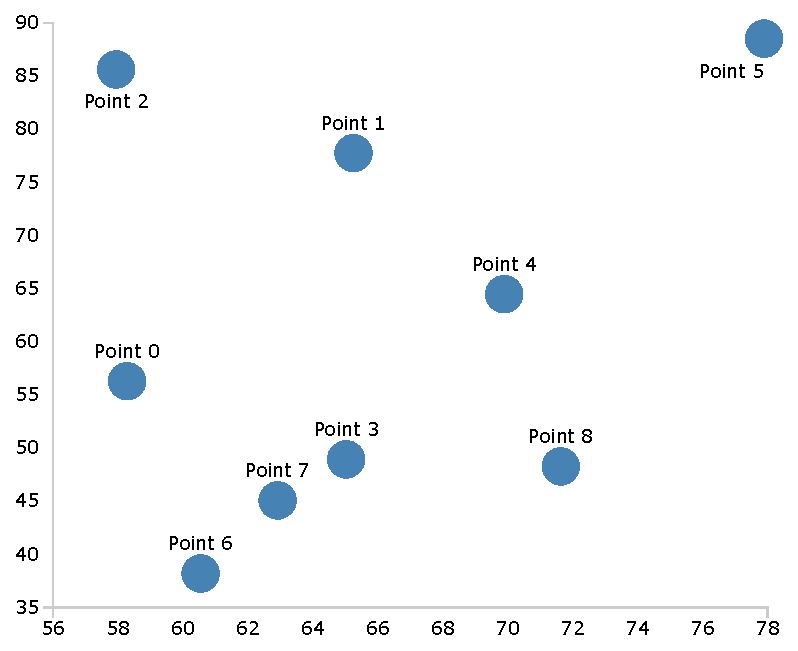
\includegraphics[width=0.3\linewidth]
{diagrams/resp-scatter-1.pdf}%
\label{fig:RespScatterExample1}%
}
\hfill
\subfloat[][%
Medium density % (0.0007 points per pixel).
]
{%
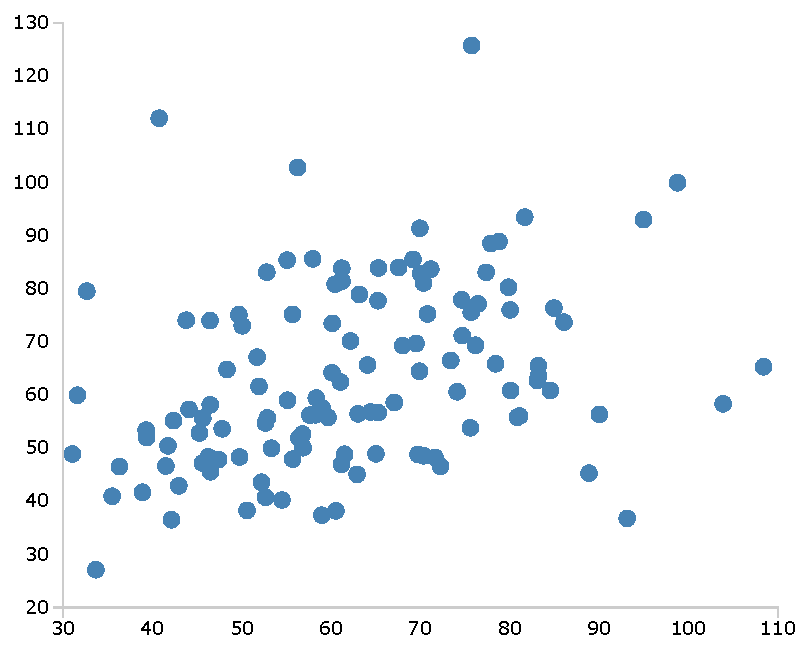
\includegraphics[width=0.3\linewidth]
{diagrams/resp-scatter-2.pdf}%
\label{fig:RespScatterExample2}%
}
\hfill
\subfloat[][%
High density % (0.017 points per pixel).
]
{%
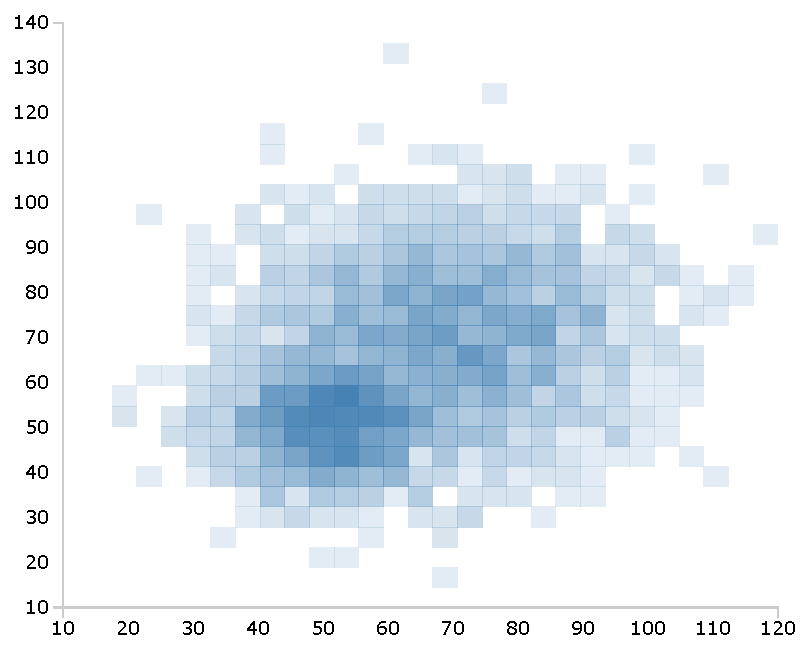
\includegraphics[width=0.3\linewidth]
{diagrams/resp-scatter-3.pdf}%
\label{fig:RespScatterExample3}%
}
\caption[Responsive Point Chart Example]
{
A responsive point chart based on data density (data
points per pixel). \subref{fig:RespScatterExample1} With a small
number of data points, all points and their corresponding labels are
shown. \subref{fig:RespScatterExample2} At a certain density, labels
are only shown for selected points. \subref{fig:RespScatterExample3}
At very high densities, the point chart is replaced by a heatmap to
more efficiently display the large amount of data.
\imgcredit{Screenshots created by the author of this thesis.
Visualization created by \textcite{NickRabinowitzRDV}}
}
\label{fig:RespScatterExample}
\end{figure}


\subsection{Parallel Coordinates}

Even though parallel coordinates charts
\parencite{ParallelCoordinates} are rarely encountered in
non-technical contexts, they are quite popular when it comes to
visualizing multidimensional data in visual analytics systems
\parencite{HighD}. In these kinds of charts, multiple dimensions are
rendered as parallel axes, upon which points are connected via paths
(polylines). Each polyline represents a data record and its values at
the corresponding dimensions. The axes of a parallel coordinates chart
are typically laid out horizontally, meaning that the chart can be
made narrower by reducing the distance between individual axes.
Previously mentioned axis-related responsive patterns, such as
rotating labels and recomposing ticks, can also be applied.

Another technique is to temporarily hide some dimensions, based on
some criteria. When automatically hiding dimensions, it is necessary
to apply compensation patterns, giving the user additional controls to
configure which dimensions are displayed and override the system's
hiding behavior. An example of a responsive parallel coordinates chart
incorporating some of these patterns can be seen in
Figure~\ref{fig:RespParCoordExample}.
%
If reducing the chart's complexity is not appropriate, an alternative
is to transpose the chart, so its dimensions are laid out vertically
and vertical scrolling can be used to explore the full chart.




\begin{figure}[tp]
\newcommand{\respparcoordscale}{0.36}
\centering
\subfloat[][%
61rem
]
{%
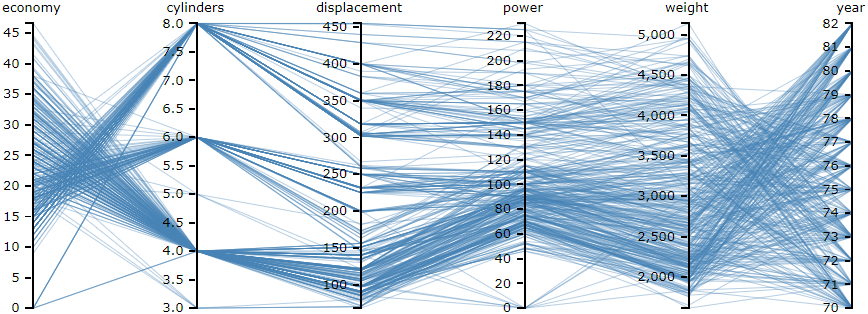
\includegraphics[valign=b,scale=\respparcoordscale]
{images/resp-parcoord-1.png}%
\label{fig:RespParCoordExample1}%
}
\hfill
\subfloat[][%
50rem
]
{%
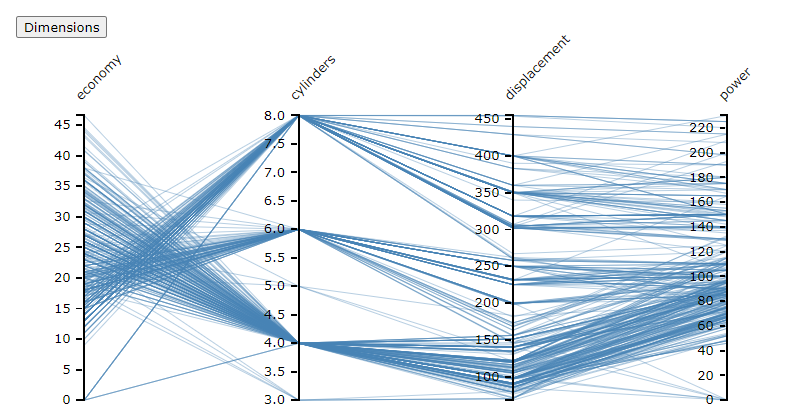
\includegraphics[valign=b,scale=\respparcoordscale]
{images/resp-parcoord-2.png}%
\label{fig:RespParCoordExample2}%
}
\newline
\subfloat[][%
40rem
]
{%
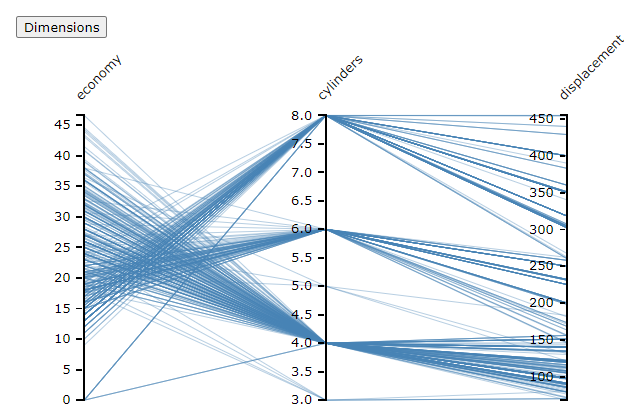
\includegraphics[valign=b,scale=\respparcoordscale]
{images/resp-parcoord-3.png}%
\label{fig:RespParCoordExample3}%
}
\hfill
\subfloat[][%
30rem
]
{%
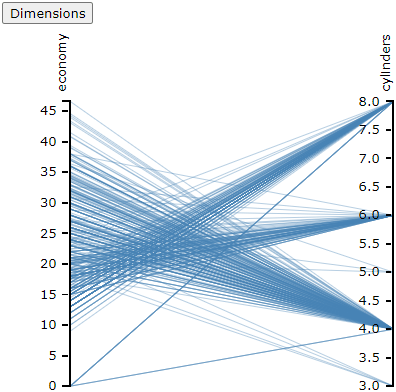
\includegraphics[valign=b,scale=\respparcoordscale]
{images/resp-parcoord-4.png}%
\label{fig:RespParCoordExample4}%
}
\hfill
\subfloat[][%
30rem, user-configured dimensions
]
{%
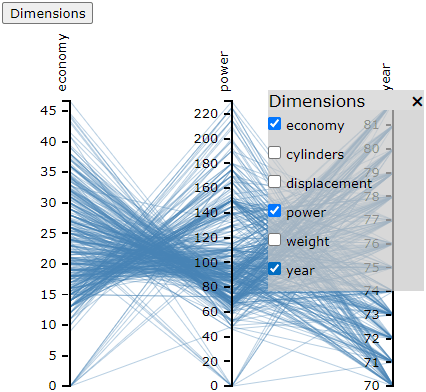
\includegraphics[valign=b,scale=\respparcoordscale]
{images/resp-parcoord-5.png}%
\label{fig:RespParCoordExample5}%
}
\caption[Responsive Parallel Coordinates Chart Example]
{
A responsive parallel coordinates chart at different display widths.
\subref{fig:RespParCoordExample1} At larger widths, all dimensions are
shown. \subref{fig:RespParCoordExample2} Dimensions are removed based
on their priority, dimension labels are rotated by 45 degrees, and a
dimensions toggle is shown which enables the configuration of
dimensions. \subref{fig:RespParCoordExample3} Further dimensions are
removed. \subref{fig:RespParCoordExample4} Further dimensions are
removed, and dimension labels are rotated by 90 degrees.
\subref{fig:RespParCoordExample5} The dimension configuration panel
has been opened, and the user has taken control over which dimensions
to show.
\imgcredit{Screenshots of \textcite{RespVis} created by the author of this thesis.
Used with kind permission by Keith Andrews.}
}
\label{fig:RespParCoordExample}
\end{figure}

